%%% use twocolumn and 10pt options with the asme2ej format
\documentclass[10pt,cleanfoot]{asme2ej}

%%% Loading packages
\usepackage{graphicx} %% for loading jpgs
\usepackage{epsfig} %% for loading postscript figures
\usepackage{fixltx2e}
\usepackage{amsmath}
\usepackage{amsfonts}
\usepackage{cite}
\usepackage{array}
\usepackage{booktabs}
\usepackage{mathtools}
\usepackage{tabularx}
%\usepackage{subfig}
\usepackage{fancyhdr}
\usepackage{setspace}
%\usepackage{helvet}
\usepackage[hyphens]{url}
\usepackage[font=small,labelfont=bf,tableposition=top]{caption}
\usepackage{subcaption}

\graphicspath{ {./images/} }
\newcommand{\hquad}{\hspace{0.5em}}
\newcommand\abs[1]{\left|#1\right|}
\newcommand\norm[1]{\left\lVert#1\right\rVert}
\renewcommand{\familydefault}{\sfdefault}
\pagestyle{fancy}
\lhead{{\it Insert ASME Journal Title in the Header Here}}
\rhead{}
\renewcommand{\headrulewidth}{0pt}
\topmargin 70 pt
\headheight 14 pt
\headsep 30 pt



\DeclareCaptionLabelFormat{andtable}{#1~#2  \&  \tablename~\thetable}
%% The class has several options
%  onecolumn/twocolumn - format for one or two columns per page
%  10pt/11pt/12pt - use 10, 11, or 12 point font
%  oneside/twoside - format for oneside/twosided printing
%  final/draft - format for final/draft copy
%  cleanfoot - take out copyright info in footer leave page number
%  cleanhead - take out the conference banner on the title page
%  titlepage/notitlepage - put in titlepage or leave out titlepage
%  
%% The default is oneside, onecolumn, 10pt, final


\title{On the synthesis and design of a novel backdrivable high-stiffness capstan drive}

%%% first author
\author{Jordan M. Longval and Clément Gosselin
    \affiliation{
    Département de génie mécanique\\
	Université Laval\\
	1065 Avenue de la Médecine\\
	Québec, Qc G1V0A6\\
	Canada\\
	Jordan.Longval.1@ulaval.ca, Clement.Gosselin@gmc.ulaval.ca
    }	
}
   

\begin{document}
\maketitle    

%%%%%%%%%%%%%%%%%%%%%%%%%%%%%%%%%%%%%%%%%%%%%%%%%%%%%%%%%%%%%%%%%%%%%%
\begin{abstract}
{\it This article introduces a novel backdrivable high-stiffness cable capstan drive architecture for robotics applications. The drive has a low transmission ratio and a higher stiffness than typical capstan drives. The higher transmission stiffness is obtained by the use of grooves on both the input and the output pulleys of the drive which increases the effective coefficient of friction between the pulleys and the cable. The groove on the input pulley forms a single helix while the grooves on the output pulley form a $R$-helix, where $R$ is equal to the transmission ratio of the drive. This property enables several different multi-cable arrangements for the drive, which further increases the transmission stiffness. A kinematic model of the capstan drive is established and used to ensure the proper alignment of the input pulley groove and output pulley grooves as a function of the distance between the pulleys. A 3D-printed prototype of the transmission is presented.
}
\end{abstract}

%%%%%%%%%%%%%%%%%%%%%%%%%%%%%%%%%%%%%%%%%%%%%%%%%%%%%%%%%%%%%%%%%%%%%%
%%%%%%%%%%%%%%%%%%%%%%%%%%%%%%%%%%%%%%%%%%%%%%%%%%%%%%%%%%%%%%%%%%%%%%
\section{Introduction}
Robotic manipulators typically use transmissions with large reduction ratios in order to reduce the size and mass of the actuators. Such transmissions (e.g. harmonic drives) are not backdrivable, which is a limitation in some applications. For example, in Collaborative Robots (CR), it is desired to provide physical Human-Robot Interaction (pHRI), i.e., to allow users to manipulate the robot links directly. 
\par 
Because their transmissions are not backdrivable, most CR used nowadays require force sensors to enable task teaching through pHRI. The force sensors are either placed near the CR's end effector \cite{roveda2018high}\cite{meissner2018smart}\cite{raessa2019teaching} or inside each joint of the CR through the use of strain gauges \cite{loughlin2007dlr}. The use of force/torque sensors limits the bandwidth of the pHRI and makes the interaction less intuitive and agile. 
\par
It is possible to teach CR tasks through pHRI without using force sensors. To this end, alternative robot kinematic architectures coupled with backdrivable Low-Ratio Transmissions (LRT) can be used. Alternative robot kinematic architectures can be used to move the CR actuators toward the base in order to minimize the influence of their inertia on the robot dynamics and payload capabilities while allowing larger and stronger actuators with backdrivable transmissions. This concept is already used in industrial palletizing  robots \cite{xiaoqing2011mechanical}, haptic devices \cite{phantom}  and backdrivable pHRI robots \cite{wen2019kinematically}\cite{9306904}. 

LRT are already used in haptic devices for telesurgery \cite{gosselin2011specification}\cite{perret2014advantages}\cite{baumann1998haptic}\cite{carignan2000closed}. Yet, not all LRT are mechanically backdrivable. For example, a worm gear cannot be driven by its output (through the worm).Table \ref{tab:LRT} shows a list of backdrivable LRT and indicates their advantages and disadvantages for pHRI.
\begin{table}[]
\centering
\caption{Comparison of different backdrivable LRT.}
\label{tab:LRT}
\begin{tabularx}{0.5\columnwidth}{@{}XXX@{}}
\toprule
LRT type    & Advantages     & Disadvantages                                                                                       \\ \midrule
Spur and helical gears &
  \begin{tabular}[c]{@{}X@{}}High stiffness\\ High torque capability\end{tabular} &
  \begin{tabular}[c]{@{}X@{}}Clearance between\\ teeth\\ (backlash)\end{tabular} \\
\hline
Belt drive &
  \begin{tabular}[c]{@{}X@{}}Transmission over a larger distance\\ No backlash\end{tabular} &
  \begin{tabular}[c]{@{}X@{}}Lower stiffness\\ Slip error\end{tabular} \\
\hline
Chain Drive & High stiffness & \begin{tabular}[c]{@{}X@{}}Clearance between inner links\\ Higher transmission inertia\end{tabular} \\
\hline
Cable (capstan drive) &
  \begin{tabular}[c]{@{}X@{}}Higher stiffness than belt drive\\ No backlash\end{tabular} &
  \begin{tabular}[c]{@{}X@{}}Lower stiffness than chain and gears\\ Slip error\end{tabular} \\ \bottomrule
\end{tabularx}
\end{table}
\par Table \ref{tab:LRT} shows that a capstan drive is a good choice of backdrivable LRT because it has higher stiffness than a belt drive and it has a lower backlash than gears or chain drives. This is why it is used in haptic devices \cite{perret2014advantages}\cite{baser2013kinematic}, highly backdrivable collaborative robots \cite{townsend1988effect}\cite{rooks2006harmonious}\cite{phan2014guided} and high precision targeting systems \cite{lu2015development}\cite{lu2012non}\cite{lu2013transmission}\cite{xie2019analytical}. Having low backlash is very important for  robotics applications which require the robot's motors to work in both directions at a high frequency \cite{brooks1990telerobotic}\cite{gealy2019quasi}. However, Table \ref{tab:LRT} also shows that capstan drives have lower stiffness than other LRT such as gears and can be subject to slip error \cite{lu2013transmission}\cite{baser2010theoretical}.\par
In order to alleviate these drawbacks, this article presents a novel capstan architecture that increases the stiffness of the transmission by using grooves on the transmission's pulleys. The grooves increase the effective friction coefficient between the cable and the pulleys, which makes the transmission stiffer. This concept has already been used in cable transmissions for elevators as described in \cite{elevator_german} and \cite{elevator}. Moreover, the novel capstan drive allows multiple cable arrangements, which further increases the stiffness of the transmission.\par This paper is structured as follows. In Sections 2 and 3, the general modelling of a capstan drive and its torsional stiffness are recalled. The theoretical model used here is based on the work of Werkmeister et al.\cite{werkmeister2007theoretical}. Part of this model is also used in \cite{baser2010theoretical}. Section 4 discusses the fact that grooves etched along the surface of a capstan drive's pulleys can theoretically increase the effective friction coefficient between the drive's cable and its pulleys thus increasing the overall stiffness of the capstan drive. This effect has been discussed in different reference books such as \cite{elevator_german} and \cite{elevator}. The result of an experiment that validates this effect is also presented in  Section 4. The use of grooves in capstan drives has already been presented in \cite{lu2012non}. However, this paper presents a novel design for the output pulley of a capstan drive which uses grooves arranged as a multiple helix. The novel design enables different multi-cable arrangements of the capstan drive that can theoretically further increase its torsional stiffness. The novel capstan drive architecture as well as different possible cable arrangements are presented in Section 5. The advantages and disadvantages  of each of the proposed arrangements are discussed. Section 6 then proposes a method to properly arrange the capstan drive's pulleys during the drive's assembly so that the cables can follow a smooth and continuous path while passing from one pulley to the other while avoiding cable interference. Section 7 shows that it is always possible to avoid two cables interfering with one another if the distance between the pulleys is large enough. A video presenting the operation of a 3D-printed prototype is introduced in Section 8. Finally, concluding remarks are made in Section 9.
\section{Modelling of a capstan drive}
Figure \ref{fig:model_capstan} presents the different elements of the capstan drive model.
\begin{figure}
    \centering
    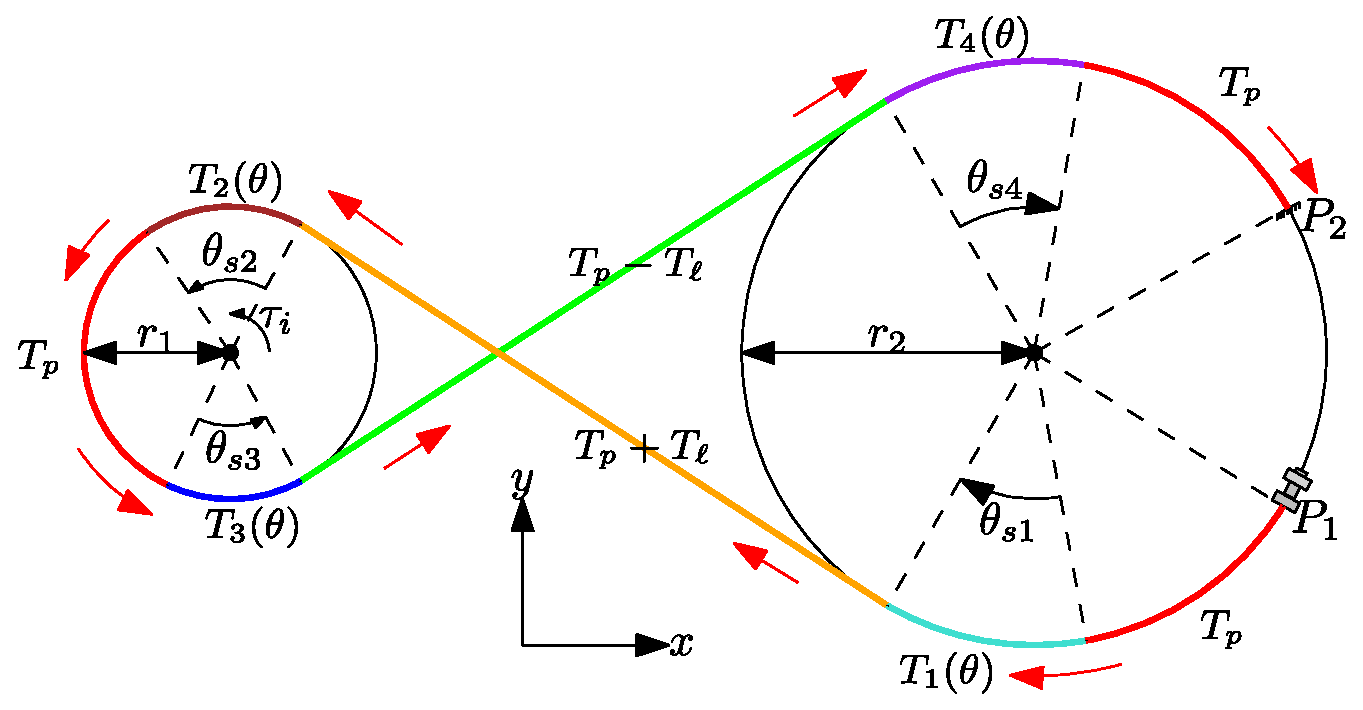
\includegraphics[width=0.5\columnwidth]{modelling_of_capstan_drive.eps}
    \caption{Modelling of a capstan drive.}
    \label{fig:model_capstan}
\end{figure}
In figure \ref{fig:model_capstan}, $r_1$ is the radius of the small input pulley while $r_2$ is the radius of the large output pulley. The transmission ratio is given by $R = \frac{r_2}{r_1}$. The cable passes from the large pulley to the small pulley and back to the large pulley in a lemniscate shaped pattern indicated by the red arrows in figure \ref{fig:model_capstan}. A preload tension $T_p$ is applied on the cable by pulling on the cable with a mechanism alike a turnbuckle (at point $P_1$) and by fixing the other end of the cable to the pulley(at point $P_2$).\par
When a torque $\tau_i$ is applied on the input pulley, one side of the cable extends while the other part of the cable shortens. The extension is caused by an increase in the tension in the cable by an amount $T_\ell$ while the contraction of the other part of the cable is caused by a reduction of the tension by an equal amount $T_\ell$. The tension on the taught side becomes $T_p+T_\ell$ while the tension on the loose side becomes $T_p-T_\ell$. The torque balance equation about the axis of rotation of the input pulley can be written as
\begin{align}
    \tau_i - (T_p+T_\ell)r_1 + (T_p-T_\ell)r_1 = 0, \label{eq:first_equation_p0}
\end{align}
which yields
\begin{align}
T_\ell = \frac{\tau_i}{2r_1}.
\label{eq:first_equation}
\end{align}
\par
The tension variations in the cable occur in contact regions between the cable and the pulleys called the slip regions. These regions are represented in figure \ref{fig:model_capstan} with the angles $\theta_{s1}$ to $\theta_{s4}$. Along these slip regions, the cable elongates or shortens due to the applied torque. This local variation in length causes friction between the pulleys and the cable. Figure \ref{fig:friction_fig} illustrates this principle. 
\begin{figure}
    \centering
    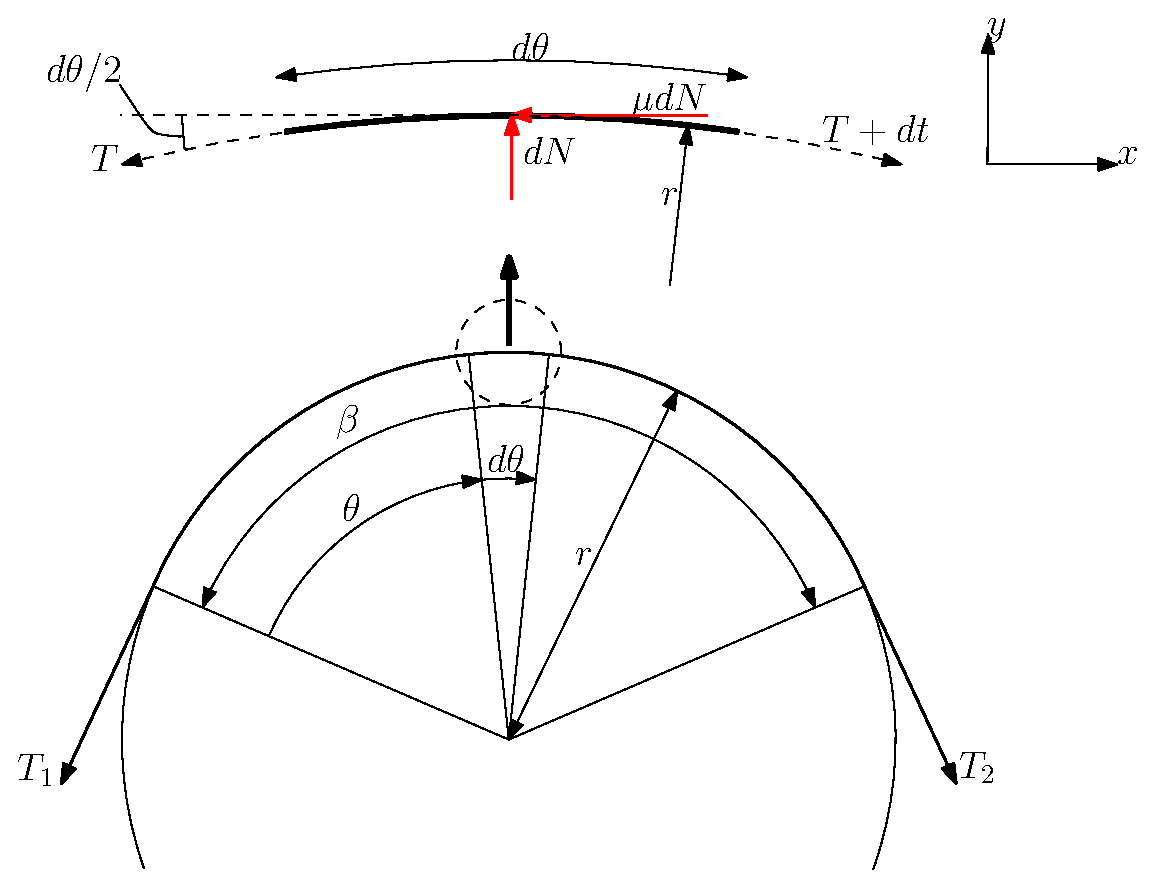
\includegraphics[width = 0.5\columnwidth]{capstan_equation.eps}
    \caption{Small segment of the cable pulley interaction.}
    \label{fig:friction_fig}
\end{figure}
\par
Figure \ref{fig:friction_fig} shows a small  segment of a cable lying on the surface of a pulley of radius $r$. The small cable segment is lying on a small angle segment of the pulley $d\theta$. The static friction coefficient between the pulley and the cable is $\mu$. The tension on one end of the small cable segment is $T$ while it is $T+dT$ at the other end. The small tension variation is created by an applied torque on the pulley. The normal force between the small cable segment and the pulley  is $dN$. When torque is applied to the pulley, the pulley surface creates a friction force on the cable segment of $\mu dN$ in the tangential direction of the torque. Calculating the force balance on the cable segment gives 
\begin{align}
    \sum F_x = T\cos\left(\frac{d\theta}{2}\right) - (T+dT)\cos\left(\frac{d\theta}{2}\right) + \mu dN =0,\label{eq:sum_f_x}\\
    \sum F_y = -T\sin\left(\frac{d\theta}{2}\right)-(T+dT)\sin\left(\frac{d\theta}{2}\right)+dN = 0.\label{eq:sum_f_y}
\end{align}
Since $d\theta$ is a small angle and $dT$ is a small tension variation, the following approximations can be made
\begin{align}
    \sin\left(\frac{d\theta}{2}\right)\approx \frac{d\theta}{2},\hquad \cos\left(\frac{d\theta}{2}\right)\approx 1,\hquad dTd\theta \approx 0. 
\end{align}
Applying these approximations to\eqref{eq:sum_f_x} and \eqref{eq:sum_f_y} gives
\begin{align}
    \frac{dT}{T} = \mu d\theta. \label{eq:diff}
\end{align}
In figure \ref{fig:friction_fig}, when the tension varies from $T_1$ to $T_2$ where $T_2>T_1$, the integration of \eqref{eq:diff} over the angle $\beta$  gives
\begin{align} 
\beta = \frac{1}{\mu}\ln\left(\frac{T_2}{T_1}\right).
\label{eq:int_beta}
\end{align}
Angle $\beta$ is referred to as the slip angle of the slip region. Integrating from $T_1$ to a function $T(\theta)$ over the slip region then gives \begin{align}
T(\theta) = T_1e^{\mu\theta},\hquad 0<\theta<\beta.\label{eq:tens_increase}
\end{align}
The same can be said by integrating from the max tension $T_2$ to a smaller tension $T(\theta)$ over the slip region $\beta$, which gives
\begin{align}
T(\theta) = T_2e^{-\mu\theta},\hquad 0<\theta<\beta.\label{eq:tens_decrease}
\end{align}
Applying \eqref{eq:int_beta}, \eqref{eq:tens_increase} and \eqref{eq:tens_decrease} to the slip regions in figure \ref{fig:model_capstan}, one finds
\begin{align}
    T_1(\theta) = T_pe^{\mu\theta},\hquad 0<\theta<\theta_{s1},\hquad \theta_{s1} = \frac{1}{\mu}\ln\left(\frac{T_p+T_\ell}{T_p}\right),\label{eq:Tens1}\\
    T_2(\theta) = (T_p+T_\ell)e^{-\mu\theta},\hquad 0<\theta<\theta_{s2},\hquad \theta_{s2}=\theta_{s1},\label{eq:Tens2}\\
    T_3(\theta) = T_pe^{-\mu\theta},\hquad 0<\theta<\theta_{s3},\hquad \theta_{s3} = \frac{1}{\mu}\ln\left(\frac{T_p}{T_p-T_\ell}\right),\label{eq:Tens3}\\
    T_4(\theta) = (T_p-T_\ell)e^{\mu\theta},\hquad 0<\theta<\theta_{s4},\hquad \theta_{s4} = \theta_{s3}.\label{eq:Tens4}
\end{align}
Equations \eqref{eq:Tens1} to \eqref{eq:Tens4} describe the variation of the tension along the cable. These equations are used in the following section to model the stiffness of a capstan drive.
%%%%%%%%%%%%%%%%%%%%%%%%%%%%%%%%%%%%%%%%%%%%%%%%%%%%%%%%%%%%%%%%%%%%%%
\section{Stiffness model of a capstan drive}
Hooke's law gives the relationship between the tensile force in an elastic object and its strain. The strain of an elastic object is also defined as its variation in length over its original length. Expressing this definition of strain in an infinitesimal form and equating it to Hooke's law, one can then write
\begin{align}
\epsilon \equiv \frac{d\delta}{dL} = \frac{F}{AE}, \Rightarrow d\delta = \frac{FdL}{AE}
\label{eq:complete_short}
\end{align}
where $\epsilon$ is the strain, $d\delta$ is a very small length variation, $dL$ is a very small cable length, $F$ is the tensile force applied on the elastic object, $A$ is the object's  cross section area and $E$ is its Young modulus. Equation \eqref{eq:complete_short} can be integrated to determine the cable deformation.
\par
The  cable deformation $\delta_i$ along the slip region $\theta_{si}$ is equal to the total deformation along the slip region minus the initial deformation caused by the preload.  Using \eqref{eq:complete_short} and using the fact that $dL=rd\theta$, the deformations $\delta_i$ are obtained as 
\begin{align}
    \delta_i = \frac{r}{AE}\left(\int_0^{\theta_{si}}T_i(\theta)d\theta-T_p\int_0^{\theta_{si}}d\theta\right),\hquad i=1,\ldots ,4 \label{eq:int_deform_i_theta}
\end{align}
where $r = r_2$ for $\theta_{s1}$ and $\theta_{s4}$ and $r = r_1$ for $\theta_{s2}$ and $\theta_{s3}$.
Applying \eqref{eq:int_deform_i_theta} to the slip angle $\theta_{s1}$ gives
\begin{align}
    \delta_1 = \frac{T_pr_2}{AE}\left(\int_0^{\theta_{s1}}e^{\mu\theta} d\theta-\int_0^{\theta_{s1}}d\theta\right), \\
    = \frac{T_pr_2}{AE}\left(\frac{1}{\mu}\left(e^{\mu\theta{s1}} -1\right)-\theta_{s1}\right),\\
    =\frac{r_2}{\mu AE}\left(T_\ell-T_p\ln\left(\frac{T_p+T_\ell}{T_p}\right)\right)\label{eq:defo1}.
\end{align}
Similarly for $\delta_2$ to $\delta_4$, one obtains 
\begin{align}
    \delta_2=\frac{r_1}{\mu AE}\left(T_\ell-T_p\ln\left(\frac{T_p+T_\ell}{T_p}\right)\right),\label{eq:defo2}\\
    \delta_3= \frac{r_1}{\mu AE}\left(T_\ell-T_p\ln\left(\frac{T_p}{T_p-T_\ell}\right)\right),\label{eq:defo3}\\
    \delta_4 =\frac{r_2}{\mu AE}\left(T_\ell-T_p\ln\left(\frac{T_p}{T_p-T_\ell}\right)\right).\label{eq:defo4}
\end{align}
Some cable deformation also occurs in the cable sections which are not in contact with the pulleys. These cable sections are here called the free sections and the deformation along these sections is obtained by integrating \eqref{eq:complete_short} which gives
\begin{align}
\delta_{f1} = \frac{T_p+T_\ell}{AE}\int_0^{L_f}dL=\frac{T_p+T_\ell}{AE}L_f,\label{eq:defof1}\\
\delta_{f2}=\frac{T_p-T_\ell}{AE}\int_0^{L_f}dL=\frac{T_p-T_\ell}{AE}L_f,\label{eq:defof2}
\end{align}
where $\delta_{f1}$ and $\delta_{f2}$ are the deformations on the tight and slack side respectively and $L_f$ is the length of the free parts of the cable which are not in contact with the pulleys.
\par
 The compliance of the different cable sections can be defined as the absolute value of the variation in deformation of the cable as a function of the applied load. Mathematically, this means that the compliance of the different cable sections can be obtained by differentiating the deformation expressions in \eqref{eq:defo1} to \eqref{eq:defof2} with respect to $T_\ell$. Furthermore, since compliance is the inverse of stiffness, one can easily obtain the stiffness of the different cable sections. For the slip regions, this gives
 \begin{align}
     C_{si}=\left|\frac{d\delta_{si}}{dT_\ell}\right|,\hquad i = 1,\ldots ,4,\label{eq:simple_stiff_1}\\
     \Rightarrow C_{s1} = \frac{r_2}{AE\mu}\left(\frac{T_\ell}{T_p+T_\ell}\right) = \frac{1}{K_{s1}}\\
     \Rightarrow C_{s2} = \frac{r_1}{AE\mu}\left(\frac{T_\ell}{T_p+T_\ell}\right)= \frac{1}{K_{s2}}\\
     \Rightarrow C_{s3} =
     \frac{r_1}{AE\mu}\left(\frac{T_\ell}{T_p-T_\ell}\right)= \frac{1}{K_{s3}}\\
     \Rightarrow C_{s4} =
     \frac{r_2}{AE\mu}\left(\frac{T_\ell}{T_p-T_\ell}\right)= \frac{1}{K_{s4}}.\label{eq:simple_stiff_4}
 \end{align}
 For the stiffnesses of the free sections of the cable, one obtains
 \begin{align}
     K_{f1}=K_{f2}=\frac{AE}{L_f}.
 \end{align}
 The total stiffness of the capstan transmission is obtained by combining the individual stiffnesses of the cable segments along the transmission. The stiffness elements $K_{s1},K_{f_1}$ and $K_{s2}$ form a serial combination of springs. The same can be said for $K_{s3},K_{f_2}$ and $K_{s4}$. The two serial spring groups are in parallel to one another meaning that the total stiffness of the transmission can be written as 
 \begin{align}
     K = K_1 + K_2,
 \end{align}
 where
 \begin{align}
     K_1 = \frac{1}{\frac{1}{K_{s1}}+\frac{1}{K_{f1}}+\frac{1}{K_{s2}}},\\
     K_2 = \frac{1}{\frac{1}{K_{s3}}+\frac{1}{K_{f2}}+\frac{1}{K_{s4}}}.
 \end{align}
 The total stiffness $K$ represents the linear stiffness of the transmission. Since a capstan drive is a torsional element, a better indicator of its stiffness is the drive's torsional stiffness when one of its pulleys is held rigidly. The torsional stiffness $K_t$ of the capstan drive when the small pulley is held rigidly and  a torque $\tau$ is applied on the large pulley, causing an angular displacement $\alpha$, is then given by
 \begin{align}
     \tau = K_t\alpha. \label{eq:rot_stiff}
 \end{align}
 The relationship between $K_t$ and $K$ is obtained by writing
 \begin{align}
    \frac{\tau_D}{r_2} = K\delta \label{eq:lin_stiff}\\
     \alpha = \frac{\delta}{r_2} \label{eq:rot_disp}.
 \end{align}
 Equation \eqref{eq:lin_stiff} gives the relationship between a torque $\tau$ applied on the large pulley  of radius $r_2$ and the total linear displacement $\delta$ when the small pulley is held tightly. Equation \eqref{eq:rot_disp} gives the relationship between the total linear displacement of the cable and the angular displacement $\alpha$ of the large pulley of radius $r_2$. Using these two equations with \eqref{eq:rot_stiff} yields
 \begin{align}
     K_t = Kr_2^2. 
 \end{align}
The following section shows how placing the capstan transmission's cable into grooves helps to increase the effective coefficient of friction between the cable and the pulleys and therefore the transmission's stiffness.

\section{Influence of grooves on the capstan drive stiffness}
 Analyzing the equations for the stiffness of the different cable sections of a capstan drive ((24) to (28)), one can clearly see that most of the stiffness terms are proportional to the coefficient of friction. Therefore, Increasing the coefficient of friction between the cable and the pulleys is an effective way to increase the overall stiffness of the transmission. Typically, the coefficient of friction is a property that is only dependent on the nature of the materials at the friction interface. However, like for a v-belt drive, by changing the geometry of the interface between two surfaces, it is possible to change the effective coefficient of friction. The way a circular groove interacts with a cable to increase the effective coefficient of friction has been studied many times as grooves are often used in elevator mechanical design \cite{elevator_german}\cite{elevator}\cite{gibsonfred}\cite{koshaktraction}. According to the aformentioned references, the effective coefficient of friction $\mu'$ for a circular groove is written as 
 \begin{align}
\mu' = \frac{4}{\pi}\mu, 
 \end{align}
where $\mu$ is the static coefficient of friction between the cable and a flat surface of the same material as the groove. This means that the use of grooves theoretically increases the friction between the cable and the groove by roughly 27.3 \%.
\par
An experimental setup was built to validate this concept. The experimental setup is shown in figures \ref{fig:exp_A} and \ref{fig:exp_B}. 
\begin{figure}
\centering
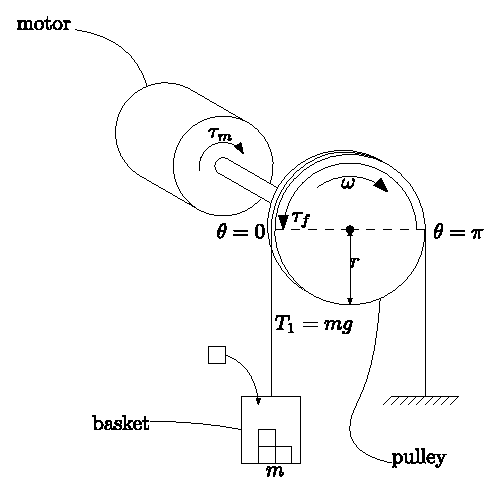
\includegraphics[width=0.5\columnwidth]{experimental_setup.eps}
\caption{Explicative illustration of the experimental setup.}
\label{fig:exp_A}
\end{figure}
In this setup, a pulley is connected to a motor which is controlled to spin at a constant speed. A rope is passed around the top half of the pulley with one end of the rope attached to a very heavy mass (immovable) and the other end of the rope attached to a basket. The cable slips on the pulley as the number of turns around the pulley (1/2) is insufficient to create traction. As more and more mass is added to the basket, the friction between the cable and the pulley increases. Therefore, a larger torque $\tau_m$ is required at the motor in order to maintain a constant speed. When the motor spins at constant speed, the torque required is equal to the total friction torque (if the internal friction torque of the motor is neglected). The total friction torque $\tau_f$, for this setup, is written as 
\begin{align}
\tau_f = r\mu\int_0^\pi dN(\theta),
\label{int_exp}
\end{align}where $r$ is the radius of the experimental pulley, $\mu$ is the friction coefficient, $dN(\theta)$ is the equivalent normal force between the cable and the pulley at the angle $\theta$ around the wrapping area. Using equations \eqref{eq:sum_f_y} and \eqref{eq:tens_decrease}, the integration in equation \eqref{int_exp} can be rewritten as 
\begin{align}
\tau_f = r\mu\int_0^\pi dN(\theta) = r\mu T_1\int_0^\pi e^{-\mu\theta}d\theta = r\mu mg\int_0^\pi e^{-\mu\theta}d\theta = rmg\left(1-e^{\mu\pi}\right).
\end{align}
In order to have a constant speed, one must have $\tau_f = \tau_m$ which means that $\mu$ can be calculated as a function of the mass of the basket $m$ and the motor torque $\tau_m$ with the following equation
\begin{align}
\mu = \frac{1}{\pi}\ln\left({\frac{rmg}{rmg-\tau_m}}\right).
\end{align} 
In the experimental setup, two pulleys of radius $r=0.03$ m were tested, one with no groove and one with a groove of the same radius as the cable in order to have a full half circled groove. The motor was spun at a constant speed of 100 RPM while the motor torque was recorded continously. The mass of the basket was progressively increased from 100 g of added mass to 900 grams of added mass (the basket having a mass of 27.6 g). The average motor torque for every mass increment was also recorded. The experiment results are presented in Table 2 and in figure 4.
\begin{figure}
\centering
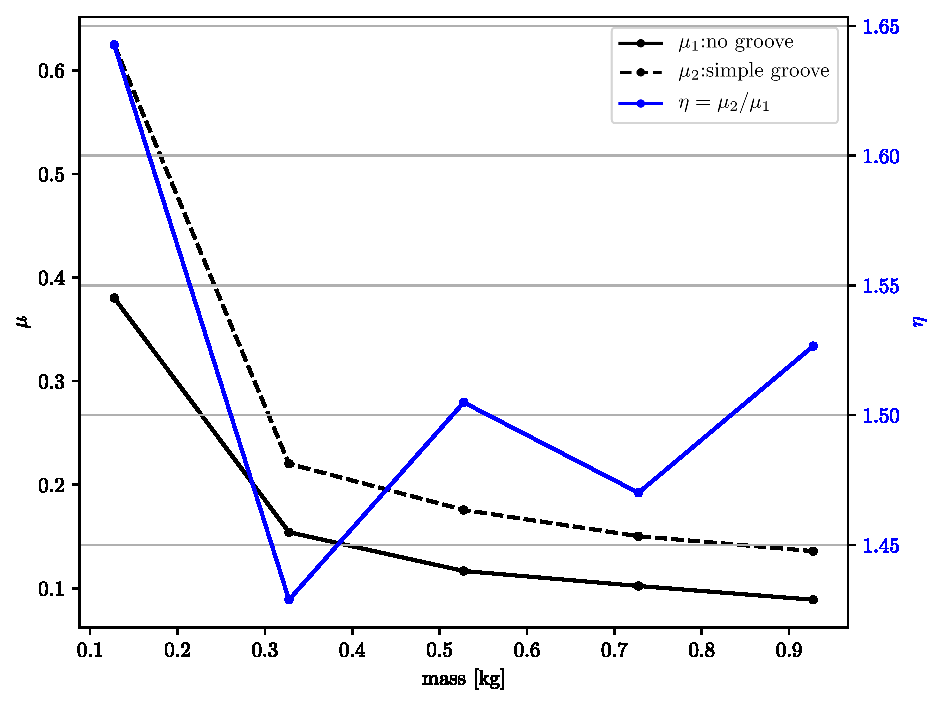
\includegraphics[width=0.47\columnwidth]{fig_exp.eps}
\qquad
\begin{tabular}[b]{cccc}\hline
      Mass [g] & $\mu_{1}$:no groove & $\mu_{2}$:simple & $\eta=\mu_{2}/\mu_{1}$\\ \hline
      127.6 & 0.38 & 0.62 & 1.64\\
      327.6 & 0.15 & 0.22 & 1.43\\
      527.6 & 0.12 & 0.18 & 1.50\\
      727.6 & 0.10 & 0.15 & 1.47\\
      927.6 & 0.09 & 0.13 & 1.53\\ \hline
      
    \end{tabular}
    \label{tab:exp_tab}
    \captionlistentry[table]{Results of the experience.}
    \captionsetup{labelformat=andtable}
    \caption{Experimental results.}
\end{figure}
\par
As it can be seen in the experimental results, the increase in the coefficient of friction when passing from no groove to a simple half circle groove is even more than what the theory predicts since the average increase is of $1.51$ times the no groove coefficient of friction. This shows that the use of grooves is indeed a good way to easily increase the coefficient of friction between the cables and the pulleys and thus increase the total stiffness of a capstan drive.
\\ 
 The following section presents a novel capstan drive architecture that takes advantage of the increased effective friction coefficient of grooved pulleys and uses multiple grooves on its output pulley in order to allow different cable arrangements which further increase the stiffness of the drive.
%%%%%%%%%%%%%%%%%%%%%%%%%%%%%%%%%%%%%%%%%%%%%%%%%%%%%%%%%%%%%%%%%%%%%
  \section{Novel capstan drive architecture}
 The novel architecture is presented in figure \ref{fig:novel_arch}. The novel capstan drive is composed of two pulleys, the input pulley of radius $r_1$ which is connected to the motor and the output pulley of radius $r_2$ which is connected to the output of the drive.  A cable indicated by a red line goes from the output pulley to the input pulley and back to the output pulley. Points $P_1$ and $P_2$ are anchoring points where the cable is fixed. The grooves on each pulley have identical cross sections. However, the groove on the input pulley forms a single helix with a pitch of $H_1$ while the grooves on the output pulley form a R-helix where $R$ is the reduction ratio of the drive, i.e. $r_2/r_1$. In figure \ref{fig:novel_arch}, the grooves on the output pulley are each indicated with a different colour to help differentiate them. Each of the output grooves has a pitch of $H_2$, where $H_2 = RH_1$.
 \begin{figure}
     \centering
     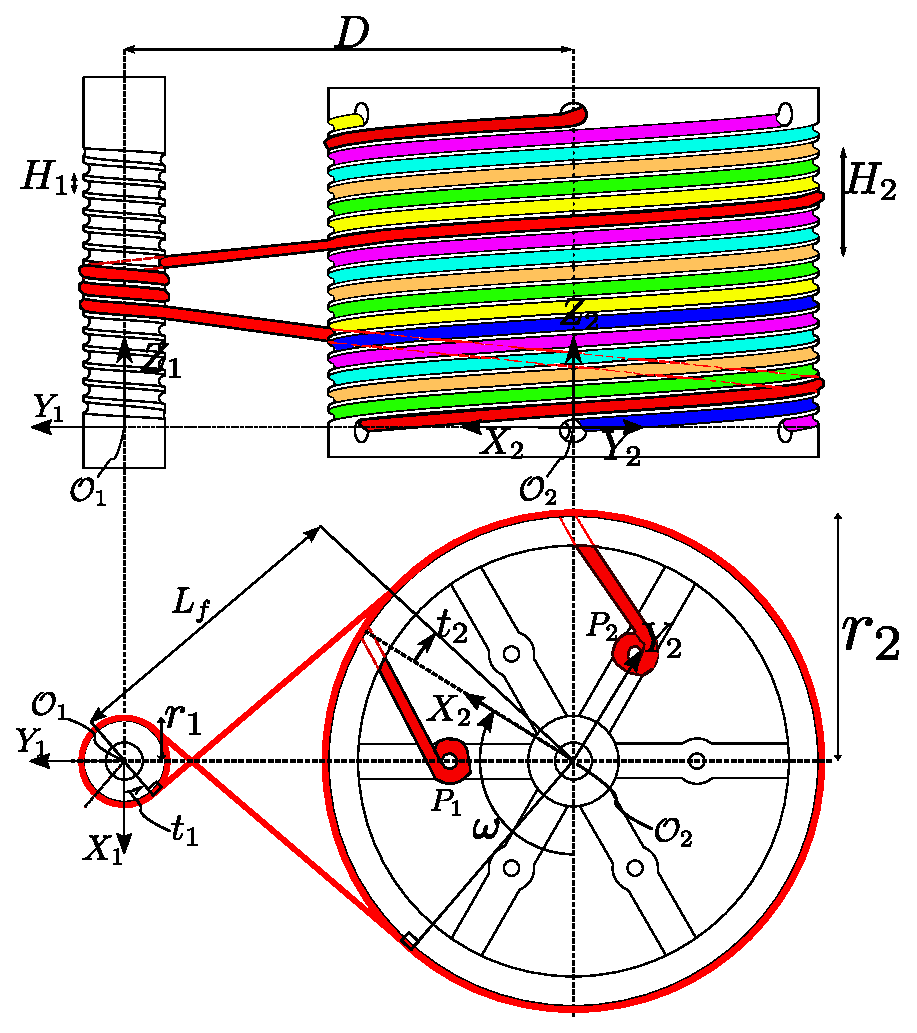
\includegraphics[width =0.3\columnwidth]{test_print_poulies.eps}
     \caption{Architecture of the novel capstan drive.}
     \label{fig:novel_arch}
 \end{figure}
 The grooves of the output pulley evolve in a direction opposite that of the grooves of the input pulley. The free cable length $L_f$ indicates the part of the cable that is not in direct contact with either of the drive pulleys. The distance between the centre axes of the pulleys is noted $D$. \\
 The presence of grooves on both the input and the output pulleys helps to increase the stiffness of the drive by increasing the effective coefficient of friction between the cable and the pulleys, as mentioned in the preceding section. Furthermore, the multiple grooves present on the output pulley enable the use of multiple cables in different cable arrangements, which can further increase the stiffness of the drive.\\
Figure \ref{fig:cable_arrangements} illustrates the different possible cable arrangements. 
 \begin{figure*}
    \centering
    \subfloat[One cable fixed at both ends to the output pulley.\label{fig:single_cable_multi_loops}]
    {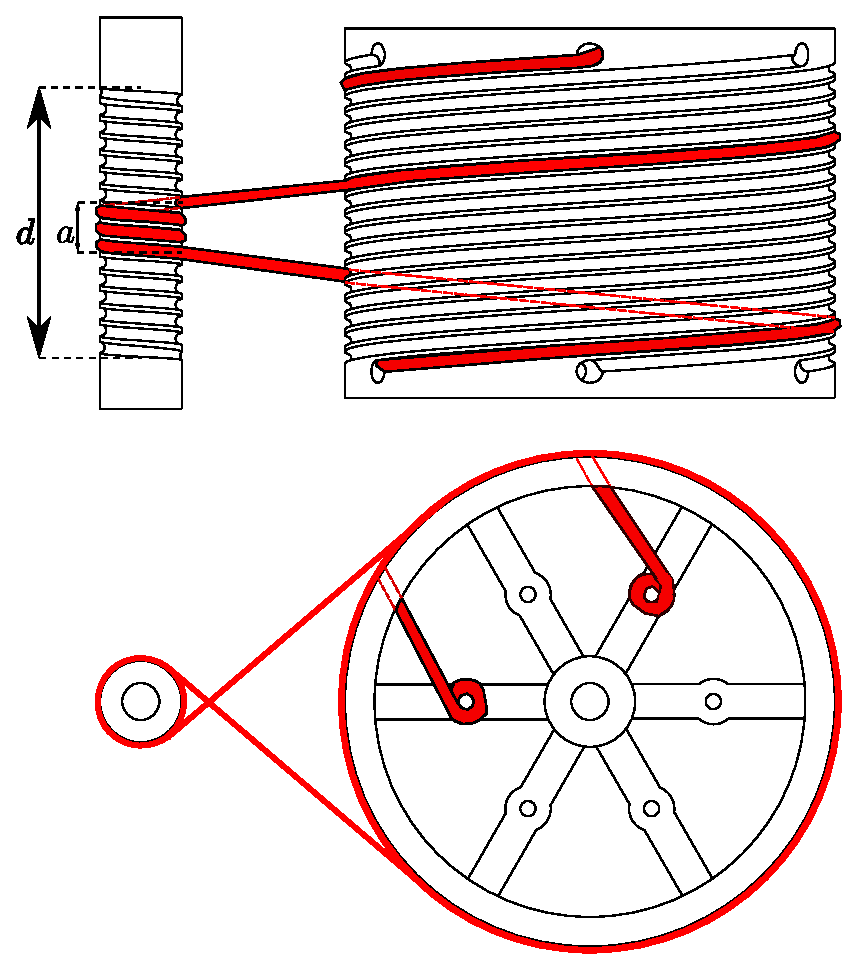
\includegraphics[width =0.3\columnwidth]{only_one_cable_multi_loops.eps}}\hspace{0.1\columnwidth}
    \subfloat[Two cables both fixed at both ends to the output pulley.\label{fig:2cables_multi_loops}]{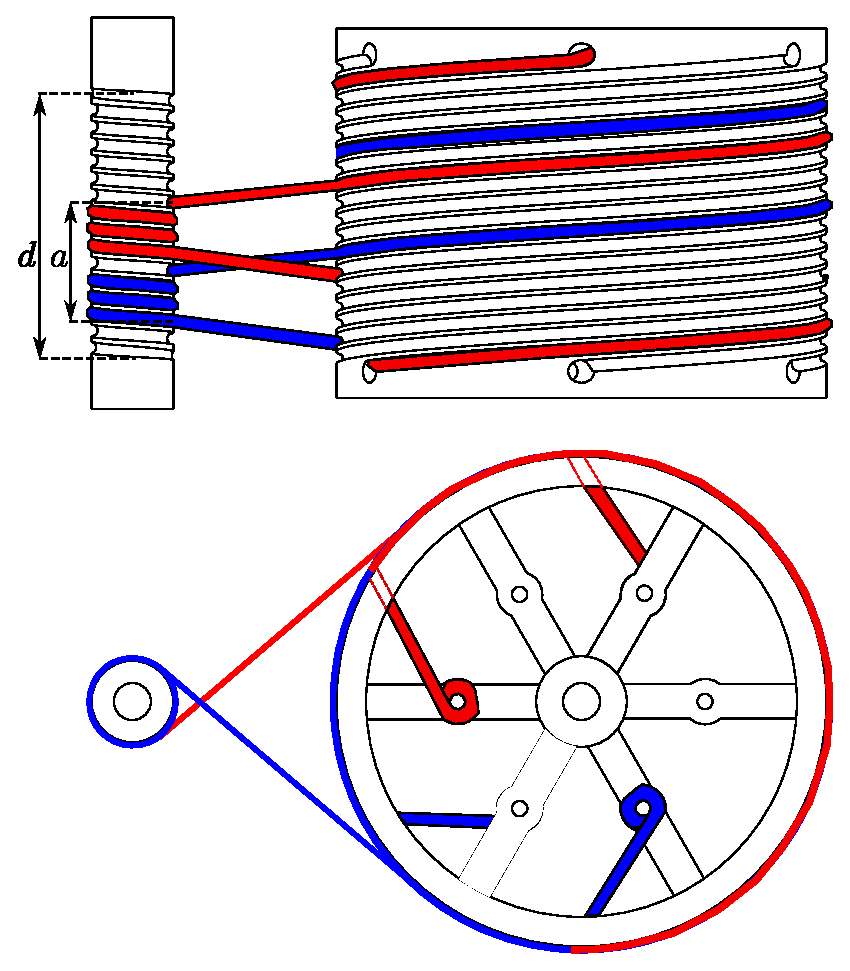
\includegraphics[width=0.3\columnwidth]{two_cables_multi_loops.eps}}
    
    \subfloat[Two cables with ends fixed at the input pulley and the output pulley.\label{fig:multi_cables_full_loops}]{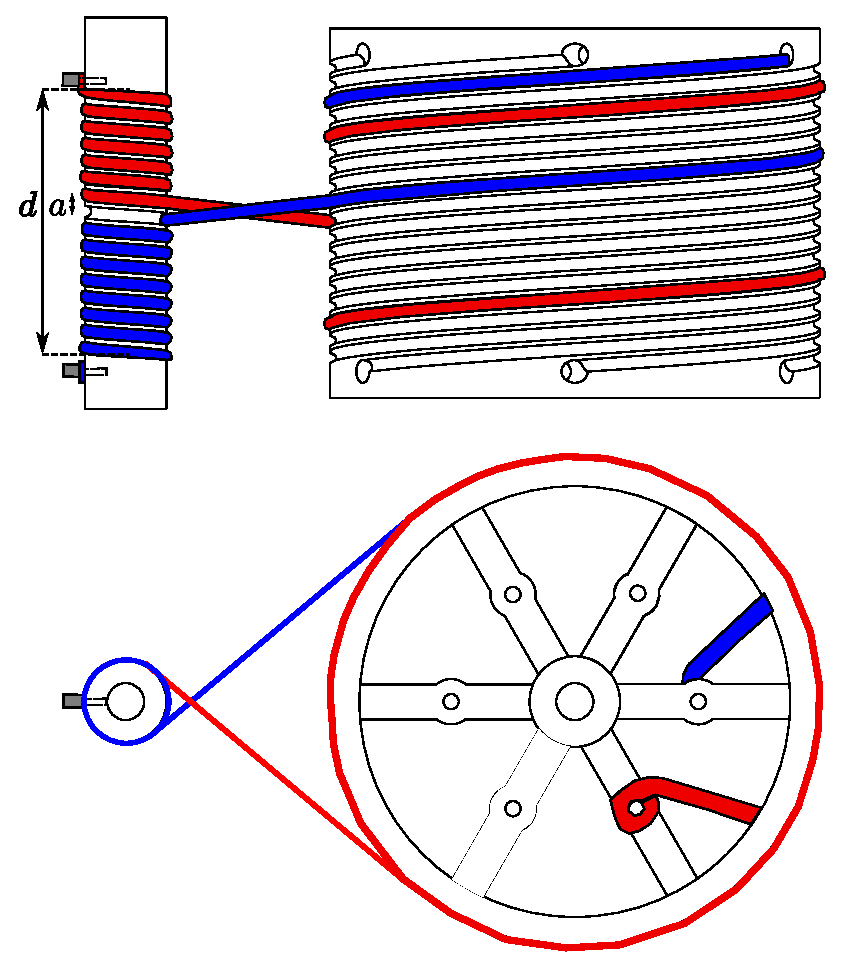
\includegraphics[width=0.3\columnwidth]{two_cables_all_loops.eps}}\hspace{0.1\columnwidth}
    \subfloat[Three cables, two having ends fixed at the input and output pulley and one being fixed at both ends to the output pulley.\label{fig:three_cables_multi_loops}]{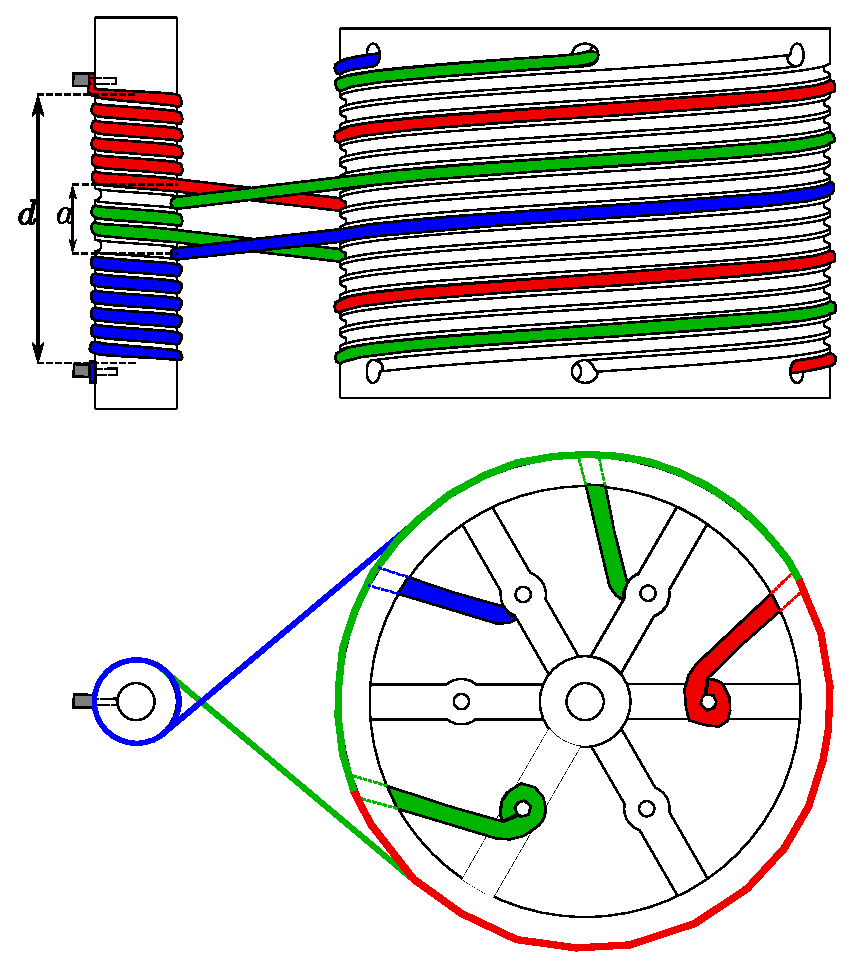
\includegraphics[width=0.3\columnwidth]{three_cables_multi_loops.eps}}
    \caption{Different possible cable arrangements.}
    \label{fig:cable_arrangements}
\end{figure*}
In figure \ref{fig:single_cable_multi_loops}, a single cable is used which is fixed at both ends to the output pulley. This arrangement has the advantage of being simple and its stiffness model is equivalent to the stiffness model of a typical capstan drive such as the one presented in figure \ref{fig:model_capstan}. This arrangement can be used many times in parallel as shown in figure \ref{fig:2cables_multi_loops} in order to multiply the total stiffness of the transmission. However, since none of the cables are fixed to the input pulley, slipping of the input pulley is possible.\\
The layout shown in figure \ref{fig:multi_cables_full_loops} uses two cables. Each cable is fixed to the input pulley at one end and to the output pulley at the other end. This cable arrangement has the advantage of ensuring that the input pulley does not slip. However, it requires two cables to obtain a transmission stiffness which is equivalent to the transmission stiffness of the single cable arrangement of figure \ref{fig:single_cable_multi_loops}.\\
The layout shown in figure  \ref{fig:three_cables_multi_loops} uses three cables. Two of its cables are fixed to both the input and output pulley while its third cable is strictly fixed to the output pulley but loops over the input pulley. The first two cables ensure the motion coupling of the input and output pulley (that there is no slipping) while the third cable helps to increase the transmission stiffness. This cable arrangement has the advantages of the two previous arrangements. \\
In all the cable arrangements shown in figure \ref{fig:cable_arrangements}, the number of turns that can be made by the output pulley is given by 
\begin{align}
N = \frac{d-a}{H_1R},
\end{align}
where  $d$ and $a$ are defined in figure \ref{fig:cable_arrangements}, $H_1$ is the pitch of the groove on the input pulley and $R$ is the reduction ratio of the drive.
In order for the cables to pass from the input pulley to the output pulley and vice versa, geometric conditions must be met in order to ensure that the helical path described by the input groove aligns with one of the helical paths of the output pulley grooves. The following section presents a mathematical model that ensures proper alignment.
\section{Alignment of the input and output grooves}
 The groove on the input pulley can best be described as a helix. The parametric helix function of the groove on the input pulley is given by 
 \begin{align}
     \mathbf{p}_1(t_1) = \begin{bmatrix}
     r_1\cos t_1\\-r_1\sin t_1\\\frac{H_1t_1}{2\pi}
     \end{bmatrix}
     \label{eq:helix_1nput}
 \end{align}
  with respect to the reference frame of the input pulley $\mathcal{O}_1$. The $X_1$ axis of $\mathcal{O}_1$ points towards the starting point of the helix. In \eqref{eq:helix_1nput},
 $t_1$ is the helix parameter of the trajectory. The second term of $\mathbf{p}_1(t_1)$ has a negative sign since the helix on the input pulley evolves in a direction opposite to the reference frame $\mathcal{O}_1$. Differentiating $\mathbf{p}_1(t_1)$ with respect to $t_1$ gives a vector that is tangent to $\mathbf{p}_1(t_1)$ and which can be written as
 \begin{align}
     \mathbf{q}_1(t_1) = \frac{d\mathbf{p}_1(t_1)}{dt_1} = \begin{bmatrix}
     -r_1\sin t_1\\-r_1\cos t_1\\\frac{H_1}{2\pi}
     \end{bmatrix}. 
 \end{align}
 The unit vector $\mathbf{u}_1(t_1)$ along $\mathbf{q}_1(t_1)$ is obtained by dividing $\mathbf{q}_1(t_1)$ by its Euclidean norm which gives
 \begin{align}
     \mathbf{u}_1(t_1) = \frac{\mathbf{q}_1(t_1)}{\rho_1}, \hquad \rho_1 = \frac{\sqrt{H_1^2+4\pi^2r_1^2}}{2\pi}.
 \end{align}
  The grooves on the output pulley can also be described by parametric helix functions. These functions can be written as
  \begin{align}
      \mathbf{p}_{2i}(t_{2i}) = \begin{bmatrix}
      r_2\cos t_{2i}\\
      r_2\sin t_{2i}\\
      \frac{H_2 t_{2i}}{2\pi}
      \end{bmatrix},\\ t_{2i} = t_2+\frac{(i-1)}{R}2\pi, \hquad i =1 ,\ldots , R,
      \label{eq:output_helix}
  \end{align}
  with respect to the reference frame of the output pulley $\mathcal{O}_2$. The $X_2$ axis points towards the starting point of one of the output grooves. In \eqref{eq:output_helix}, $t_2$ is the general helix parameter of the output pulley and the $t_{2i}$ parameters are specific to each individual groove of the output pulley. \\ 
  Differentiating vectors $\mathbf{p}_{2i}(t_{2i})$ with respect to $t_{2}$ gives vectors that are tangent to their respective $\mathbf{p}_{2i}(t_{2i})$ vectors. These tangent vectors can be written as 
  \begin{align}
      \mathbf{q}_{2i}(t_{2i}) = \frac{d \mathbf{p}_{2i}(t_{2i})}{dt_{2}}=\begin{bmatrix}
      -r_2\sin t_{2i}\\
      r_2\cos t_{2i}\\
      \frac{H_2}{2\pi}
      \end{bmatrix},\hspace{0.5em}i =1 ,\ldots , R.
  \end{align}
  The tangent unit vectors along the $\mathbf{q}_{2i}(t_{2i})$ vectors are given by
  \begin{align}
      \mathbf{u}_{2i}(t_{2i}) = \frac{\mathbf{q}_{2i}}{\rho_2},\hspace{0.5em} \rho_2 = \frac{\sqrt{H_2^2+4\pi^2r_2^2}}{2\pi}, \hspace{0.5em} i = 1 ,\ldots , R.
  \end{align}
  The helix functions of the input pulley groove and one of the output pulley grooves can be expressed as a function of one another in the following loop closure equation
  \begin{align}
      \mathbf{p}_1 + L_f\mathbf{u}_1 = \mathbf{a}+\mathbf{Q}\mathbf{p}_{2i}, \hquad i =1 ,\ldots , R,
      \label{eq:loop_closure}
  \end{align}
  where $\mathbf{a}=\begin{bmatrix}0 && -D  && 0\end{bmatrix}^T$ is a vector expressed in the $\mathcal{O}_1$ reference frame and $\mathbf{Q}$ is a rotation matrix expressing a change of reference frame from $\mathcal{O}_2$ to $\mathcal{O}_1$ and is written as \begin{align}
  \mathbf{Q} =
  \begin{bmatrix}
  \cos \omega && -\sin \omega && 0\\
  \sin \omega && \cos \omega && 0\\
  0 && 0 && 1
  \end{bmatrix},
  \end{align}
  where $\omega$ represents the amount of rotation of the output pulley needed in order to have the cables pass smoothly between the two pulleys.
  Equation \eqref{eq:loop_closure} is equivalent to the three following scalar equations
  \begin{equation}
  \begin{multlined}
      r_1\left(\cos t_1 -\frac{L_f}{\rho_1}\sin t_1\right)=r_2\cos\left(\omega+t_{2i}\right),\\ i=1 ,\ldots , R,\label{eq:loop_closure_deriv1}
      \end{multlined}
      \end{equation}
      \begin{align}
      \begin{multlined}
      -r_1\left(\sin t_1 + \frac{L_f}{\rho_1}\cos t_1\right)=-D+r_2\sin\left(\omega+t_{2i}\right),\\ i=1 ,\ldots , R,\label{eq:loop_closure_deriv2}
      \end{multlined}
      \end{align}
      \begin{equation}
      H_1\left(t_1+\frac{L_f}{\rho_1}\right) = H_2t_2.\label{eq:loop_closure_deriv3}
  \end{equation}
  In addition to these equations, in order to ensure the proper alignment of the input and output pulley grooves, one must be able to draw a straight line from the input groove to one of the output grooves where the line is tangent to both grooves. This can be mathematically written as 
  \begin{align}
      \mathbf{q}_1 \times \mathbf{Q}\mathbf{q}_{2i} = \mathbf{0},\hquad i=1 ,\ldots , R,
  \end{align}
  which is equivalent to the following three scalar equations 
  \begin{align}
      \frac{H_2r_1}{2\pi}\cos t_1 + \frac{H_1r_2}{2\pi}\cos(\omega+t_{2i})=0,\hquad i=1 ,\ldots , R,\label{eq:cross_prod_1}\\
      \frac{H_2r_1}{2\pi}\sin t_1-\frac{H_1r_2}{2\pi}\sin(\omega + t_{2i})=0,\hquad i=1 ,\ldots , R,\label{eq:cross_prod_2}\\
      \sin\left(t_1+t_{2i}+\omega\right)=0,\hquad i=1 ,\ldots , R.\label{eq:cross_prod_3}
  \end{align}
From \eqref{eq:cross_prod_3}, we obtain that
\begin{align}
    t_1+t_{2i}+\omega = n\pi, n\in \mathbb{N},\hquad i = 1,\ldots ,R.\label{eq:cross_prod_deriv1}
\end{align}
Substituting \eqref{eq:cross_prod_deriv1} into \eqref{eq:cross_prod_1} and \eqref{eq:cross_prod_2} yields
\begin{align}
    \frac{H_2r_1}{2\pi}\cos t_1 + \frac{H_1r_2}{2\pi}\cos(n\pi-t_1)=0,\hquad i=1,\ldots ,R,\label{eq:cross_prod_deriv2}\\
    \frac{H_2r_1}{2\pi}\sin t_1-\frac{H_1r_2}{2\pi}\sin( n\pi-t_1)=0,\label{eq:cross_prod_deriv3}\hquad i=1 ,\ldots , R.
\end{align}
Equations \eqref{eq:cross_prod_deriv2} and \eqref{eq:cross_prod_deriv3} are both satisfied if 
\begin{align}
    H_2r_1 = H_1r_2\label{eq:cond_cross_prod_2}
\end{align} 
and 
\begin{align}
    n = 2m+1, \hquad m \in \mathbb{N}.\label{eq:cond_cross_prod_3}
\end{align}
Equations \eqref{eq:cross_prod_deriv1}, \eqref{eq:cond_cross_prod_2} and \eqref{eq:cond_cross_prod_3} represent the conditions that must be met in order to be able to draw a straight line from the input pulley groove to one of the output pulley grooves where the line is tangent to both grooves. Substituting these conditions into \eqref{eq:loop_closure_deriv1} and \eqref{eq:loop_closure_deriv3} leads to
\begin{align}
    (r_2+r_1)\cos t_1 = \frac{L_fr_1}{\rho_1}\sin t_1,\label{eq:loop_closure_deriv4}\\
    D - \left(r_2+r_1\right)\sin t_1 = \frac{L_fr_1}{\rho_1}\cos t_1.\label{eq:loop_closure_deriv5}
\end{align}
Dividing  \eqref{eq:loop_closure_deriv4} by \eqref{eq:loop_closure_deriv5} and rearranging then yields
\begin{align}
   \sin t_1 = \left(\frac{r_2+r_1}{D}\right).\label{eq:deriv_eq_tI}
\end{align}
The right-hand side term in \eqref{eq:deriv_eq_tI} is bound between 0 and 1 since $D\in\left[(r_2+r_1),\infty \right[$. This means that 
\begin{align}
    t_1 =  \varphi + 2\pi p,\hquad p \in \mathbb{N}\label{eq:deriv_eq_tI2}
\end{align}
or 
\begin{align}
    t_1 =(2p+1)\pi-\varphi,\hquad p \in \mathbb{N},\label{eq:deriv_eq_tI3}\\
    \varphi = \sin^{-1}\left(\frac{r_1+r_2}{D}\right).
\end{align}
Substituting \eqref{eq:deriv_eq_tI3} into \eqref{eq:loop_closure_deriv4}, one finds that $L_f$ would need to have a negative length, which is impossible. This is not the case when $t_1$ is given by \eqref{eq:deriv_eq_tI2} and therefore this is the only possible value for $t_1$. The value of $L_f$ is thus
\begin{align}
L_f = \frac{\rho_1}{r_1}\sqrt{D^2-(r_2+r_1)^2}.
\label{eq:val_Lf}
\end{align}
Having $L_f$ and $t_1$, one can finally find the value of $\omega$ using \eqref{eq:loop_closure_deriv3} and \eqref{eq:cross_prod_deriv1} as 
\begin{align}
\begin{multlined}
\omega = \left(2m+1\right)\pi-t_1-\frac{\left(t_1+\frac{L_f}{\rho_1}\right)}{R}-\frac{2\pi(i-1)}{R},\\ i=1 ,\ldots , R, m \in \mathbb{N},
\label{eq:delta_def}
\end{multlined}
\end{align}
with $t_1$ given by \eqref{eq:deriv_eq_tI2} and $L_f$ given by \eqref{eq:val_Lf}. Equation \eqref{eq:delta_def} can be simplified since the output pulley is $2\pi/R$ symmetric about the $Z_2$ axis in figure \ref{fig:novel_arch}. The simplified version of \eqref{eq:delta_def} is written as
\begin{align}
\omega = \left(\frac{-\left(\varphi\left(R+1\right)+\frac{L_f}{\rho_1}\right)}{R}\right)//\left(\frac{2\pi}{R}\right),
\end{align}
where $a//b$ returns the remainder of $a$ divided by $b$.\\

Angle $\omega$ varies with the distance separating the axes of the input and output pulleys $D$. Knowing $D$, properly aligning the pulleys so that the cables follow a smooth path simply requires that both pulleys be locked during the cable mounting with the large pulley being rotated by an angle $\omega$ from the $X_1$ axis of the small pulley around the $Z_2$ axis of the large pulley. After having taught all the cables at both ends, the system can then be unlocked and the pulley grooves are properly aligned.\par
The next section shows that there exists a minimal distance between the two capstan drive pulleys to ensure that there is no cable interference.
\section{Minimal distance between pulleys to avoid cable interference.}
The cable arrangements in figures \ref{fig:multi_cables_full_loops}, \ref{fig:2cables_multi_loops} and \ref{fig:three_cables_multi_loops} all display the situation where cable interference between two distinct cables might be possible if the distance between the pulleys is too small. However, one can determine the minimal distance $D$ between the two capstan pulleys as a function of the cable diameter $\zeta$. Figure \ref{fig:cable_interference} shows a modified version of figure \ref{fig:multi_cables_full_loops} which includes a reference frame from which positions of interest can be established. 
\begin{figure}
\centering
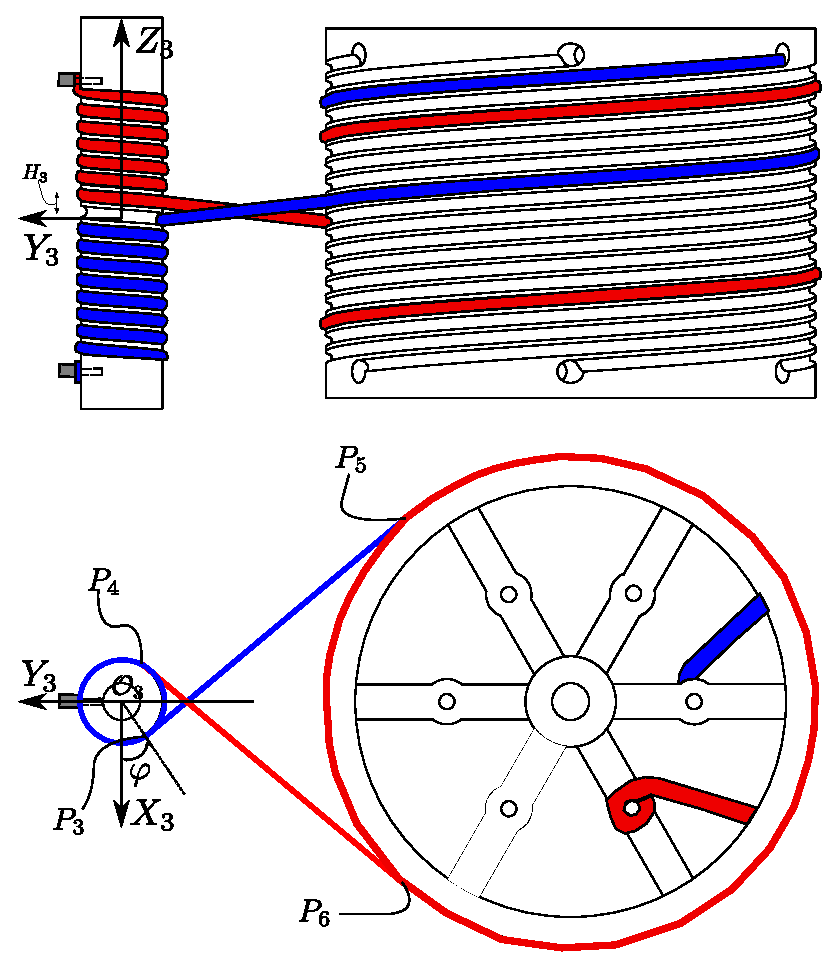
\includegraphics[width =0.5\columnwidth]{fig_cable_interference.eps}
\caption{Determining the shortest cable to cable distance in a two cable arrangement.}
\label{fig:cable_interference}
\end{figure}
 In figure \ref{fig:cable_interference}, points $P_3$ and $P_4$ are respectively the points where the blue and the red cable tangentially leave the small pulley of radius $r_3$.
The position of these points with respect to the reference frame $\mathcal{O}_3$ can be respectively written as 
\begin{align}
P_3: \mathbf{p}_3 = \begin{bmatrix}
r_3\cos\varphi\\
-r_3\sin\varphi\\
\frac{H_3}{2\pi}\varphi
\end{bmatrix},\quad P_4:\mathbf{p}_4 = \begin{bmatrix}
-r_3\cos\varphi\\
-r_3\sin\varphi\\
\frac{H_3}{2\pi}\left(3\pi-\varphi\right)
\end{bmatrix},
\end{align}
where $H_3$ is the pitch of the input pulley helix and $\varphi$ is given by
\begin{align}
\varphi = \sin^{-1}\left(\frac{r_3+r_4}{D}\right)
\end{align} where $r_3$ is the radius of the small pulley, $r_4$ is the radius of the large pulley and $D$ is the center to center distance between the two. Furthermore, the tangent unit vectors at points $P_3$ and $P_4$ pointing in the direction leaving the small pulley can be expressed respectively as 
\begin{align}
\mathbf{u}_3 = \frac{\begin{bmatrix}
-r_3\sin\varphi\\
-r_3\cos\varphi\\
\frac{H_3}{2\pi}
\end{bmatrix}}{\rho_3}, \quad \mathbf{u}_4 =\frac{\begin{bmatrix}
r_3\sin\varphi\\
-r_3\cos\varphi\\
\frac{-H_3}{2\pi}
\end{bmatrix}}{\rho_3}, \quad \rho_3 = \frac{\sqrt{H_3^2+4\pi^2r_3^2}}{2\pi}.
\end{align} 
With vectors $\mathbf{p}_3$, $\mathbf{p}_4$, $\mathbf{u}_3$ and $\mathbf{u}_4$, one can describe two lines $l_3$ and $l_4$ which are coincident with the free blue and red cable segments in fig \ref{fig:cable_interference} and which are written parametrically as
\begin{align}
l_3:\mathbf{p}(s_3) = \mathbf{p}_3 + \mathbf{u}_3s_3, \quad l_4:\mathbf{p}(s_4) = \mathbf{p}_3 + \mathbf{u}_4s_4,\quad s_3,s_4 \in \mathbb{R},
\label{eq:eq_of_two_lines}
\end{align}
where $s_3$ and $s_4$ are the parameters of the lines $l_3$ and $l_4$. It is well known that the smallest distance $d$ between two skew lines $l_A$ and $l_B$ in respective parametric equations can be obtained as \begin{align}
l_A: \mathbf{p}(s_A) = \mathbf{m}_As_A+\mathbf{b}_A,\quad l_B: \mathbf{p}(s_B) = \mathbf{m}_Bs_A+\mathbf{b}_B,\quad \Rightarrow d = \abs{\frac{\mathbf{m}_A\times\mathbf{m}_B}{\norm{\mathbf{m}_A\times\mathbf{m}_B}}\cdot\left(\mathbf{b}_B-\mathbf{b}_A\right)}.
\end{align}
Applying this equation to the parametric lines $l_3$ and $l_4$ gives
\begin{align}
d = \abs{\frac{H_3r_3\left(3\pi-2\sqrt{\gamma^2-1}-2\sin^{-1}(1/\gamma)\right)}{\sqrt{H_3^2\gamma^2+4\pi^2r_3^2}}},
\label{eq:distance_func}
\end{align}
where
\begin{align}
\gamma = \frac{D}{r_3+r_4}.
\end{align}
Finally, using equation \eqref{eq:distance_func} and replacing $d$ by the diameter $\zeta$, one can write the following condition which ensures that the cables will not touch
\begin{align}
\abs{\frac{H_3r_3\left(3\pi-2\sqrt{\gamma^2-1}-2\sin^{-1}(1/\gamma)\right)}{\sqrt{H_3^2\gamma^2+4\pi^2r_3^2}}} > \zeta.
\label{eq:ineq_dist}
\end{align}
Finding a pair $D$ and $H_3$ such that \eqref{eq:ineq_dist} is true means that cable interference will be avoided.
%This process is better illustrated in figure \ref{fig:process_align}.
%\begin{figure*}
%\centering
%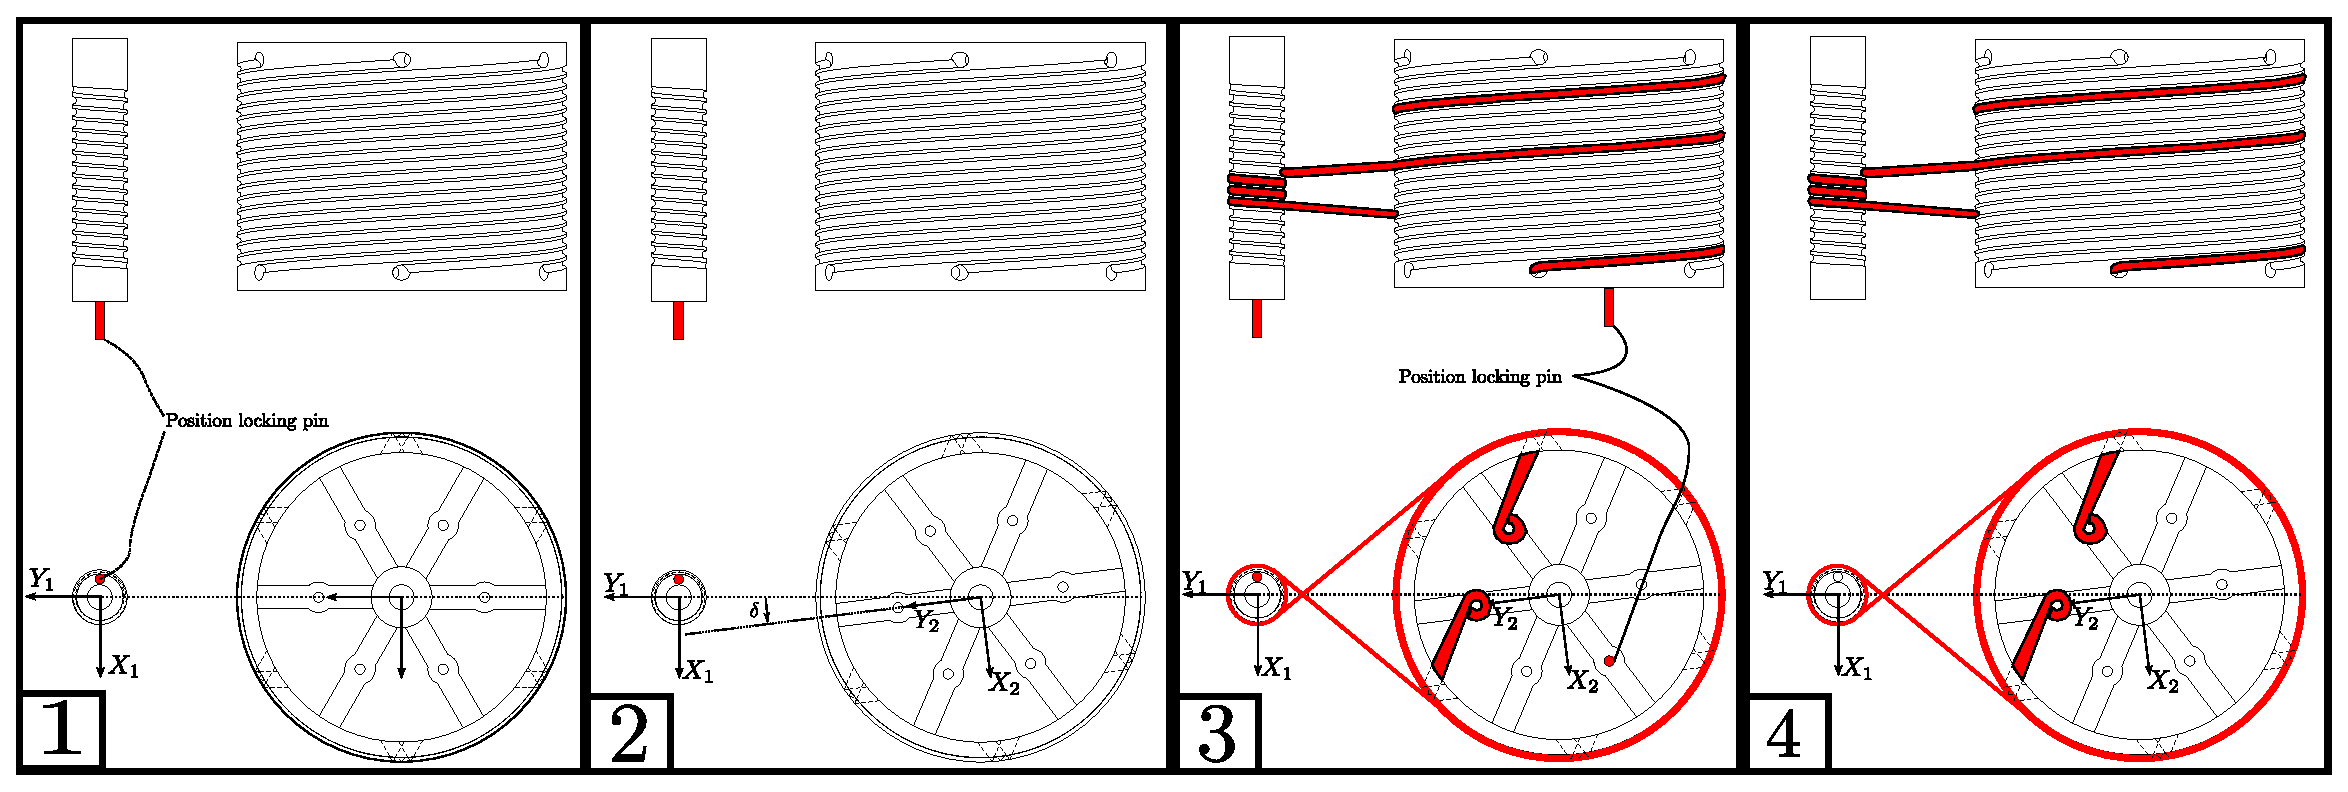
\includegraphics[width = 0.7\columnwidth]{steps.eps}
%\caption{Steps to align the drive pulleys for smooth cable %trajectories.}
%\label{fig:process_align}
%\end{figure*}
\section{Multimedia extension}
A video accompanies this paper. The video demonstrates the operation of a prototype of the novel capstan drive as well as its backdrivability.
\section{Conclusion}
This paper presented a novel capstan drive architecture which uses grooves on both its input and output pulleys in order to increase the effective coefficient of friction between the drive cables and the pulleys. Using a previously established model of a capstan drive, it was shown that increasing the coefficient of friction between the drive cables and the drive pulleys increases the drive stiffness, which is an important property in several applications, including for instance physical human-robot interaction. Furthermore, the many grooves on the output pulley enable multi-cable arrangements which can even further increase the transmission's stiffness. A method to ensure that the drive cables can pass smoothly between the input and output pulley was also described. \\
Future work on this novel capstan drive will consist in testing the established model in a test bench in order to quantify the increased coefficient of friction caused by the grooves as well as to quantify the increase in drive stiffness compared to a standard capstan drive. Furthermore, the influence of the increased drive stiffness on the drive's bandwidth will be analyzed and compared to other small-ratio transmissions in order to determine if this novel drive is advantageous for physical human robot interaction.
%%%%%%%%%%%%%%%%%%%%%%%%%%%%%%%%%%%%%%%%%%%%%%%%%%%%%%%%%%%%%%%%%%%%%%
\begin{acknowledgment}
This work was supported by the Natural Sciences and Engineering Research Council of Canada (NSERC) and by the
Canada Research Chair Program.
\end{acknowledgment}

%%%%%%%%%%%%%%%%%%%%%%%%%%%%%%%%%%%%%%%%%%%%%%%%%%%%%%%%%%%%%%%%%%%%%%
% The bibliography is stored in an external database file
% in the BibTeX format (file_name.bib).  The bibliography is
% created by the following command and it will appear in this
% position in the document. You may, of course, create your
% own bibliography by using thebibliography environment as in
%
% \begin{thebibliography}{12}
% ...
% \bibitem{itemreference} D. E. Knudsen.
% {\em 1966 World Bnus Almanac.}
% {Permafrost Press, Novosibirsk.}
% ...
% \end{thebibliography}

% Here's where you specify the bibliography style file.
% The full file name for the bibliography style file 
% used for an ASME paper is asmems4.bst.
\bibliographystyle{asmems4}

% Here's where you specify the bibliography database file.
% The full file name of the bibliography database for this
% article is asme2e.bib. The name for your database is up
% to you.
%\bibliography{asme2e}
\bibliography{./bibliography/asme2e}

\end{document}
